% !TEX encoding = UTF-8
% !TEX TS-program = pdflatex
% !TEX root = ../tesi.tex

%**************************************************************
\chapter{Conclusioni}
\label{cap:conclusioni}
%**************************************************************
%**************************************************************




\section{Raggiungimento degli obiettivi}
L'attività dello stage è terminata come previsto il 10/01/2018 senza particolari sforamenti. 
A fine stage è valutato il livello di raggiungimento degli obiettivi, dal quale tutti gli obiettivi obbligatori elencati nella tabella
4.1 risultano essere soddisfati. Gli obiettivi elencati nella tabella nonostante pochi in numero, comprendono implicitamente a loro volta altri obiettivi il quale soddisfacimento ha richiesto quantità di tempo lavorativo non trascurabile. Per quanto riguarda gli obiettivi desiderabili, è stato soddisfatto l'obiettivo con l'identificativo OB-9-D che consiste nel testare una serie di formule riassuntive dell'applicativo preesistente. E' rimasto invece non soddisfatto l'obiettivo OB-10-D a causa
 dell'esaurimento delle ore prefissate nel documento piano di lavoro.\\\\
 I seguenti grafici evidenziano un confronto tra le ore di pianificazione preventivate e quelle consuntivate. Nel secondo grafico notimo che l'attività di progettazione e sviluppo risulta essere aumentato di ore pari a venti, a causa di alcune anomalie del framework MyBatis. Queste ore sono state ammortizzate nell'attività di implementazione e testing. 
\clearpage
\begin{figure}[h]
   \begin{center}
       \caption{Ore di pianificazione preventivate}
     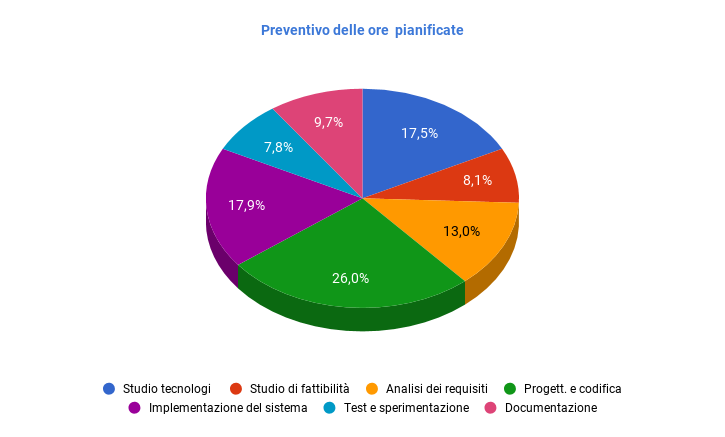
\includegraphics[scale=0.45]{diagrammi/preventivo} 

    \end{center}



   \begin{center}
     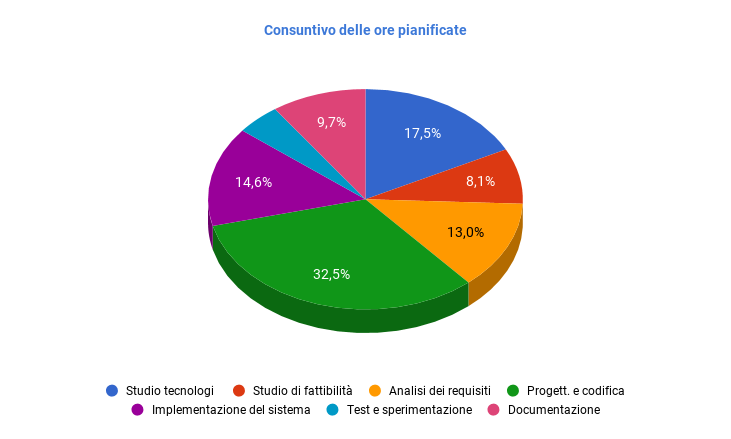
\includegraphics[scale=0.45]{diagrammi/consuntivo} 
    \caption{Ore di pianificazione consuntivate}
    \end{center}
\end{figure}

\clearpage
 
 
\begin{table}
\subsection{Alcune statistiche sull'utilizzo dell'applicativo}

La tabella seguente mostra alcune statistiche raccolte dal momento del rilascio dell'applicativo. Nella prima colonna viene riportata una media di messaggio inviati/ricevuti in una settimana per gli utenti non amministratori. La seconda colonna invece rappresenta i messaggi inviati e ricevuti dagli utenti amministratori. Quest'ultimi hanno accesso dell'area amministrativa per la gestione degli utenti registrati e in attesa. Nella terza colonna vengono riportati i tempi di risposta per operazione testati su uno smartphone con rete 4G. Come si vede dalla tabella, l'operazione che richide più tempo è la Disponibilità poichè  crea un PDF che contiene al suo interno un elevato numero di tabelle. \\




\begin{tabular}{ |p{3cm}|p{3cm}|p{3cm}|p{3cm}| }

 \hline
   & \textbf{Msg inv/ric in Sett per utente}    &  \textbf{Msg inv/ric in Sett per Admin}  &  \textbf{tempo risposta/operazione}\\ 
 \hline
  \textbf{Ordinati} &  20   & ND & 1Sec\\

 \hline
  \textbf{Scadenze} &  15   & 15 & 1Sec\\
 \hline
   \textbf{Spedito} &  30   & ND & 1Sec\\
 \hline
    \textbf{Disponibilità} &  15   & ND & 5Sec\\
 \hline
   \textbf{Inevasi} &  15   & ND & 3Sec\\
 \hline
    \textbf{Scadenzario} &  15   & 10 & 3Sec\\
 \hline
    \textbf{Amministrazione} &  ND   & 8 & 0.7Sec\\
 \hline
\end{tabular}
\\
\caption{Tabella statistiche applicativo }
\end{table}




%**************************************************************
\section{Conoscenze acquisite}
Le conoscenze acquisiste durante il periodo di stage presso l'azienda Sanmarco Informatica S.p.A. sono state significative e di grande valore. Grazie all'utilizzo dei servizi offerti da telegram per la parte back-end, ho avuto la possibilità di acquisire conoscenze più approfondite per quanto riguarda il linguaggio di programmazione Java con il suo modello di programmazione orientata agli oggetti e uno studio più approfondito legato ai suoi algoritmi implementati. Lavorando in un team composto da cinque persone sono stato in grado di comprendere quali sono le più comuni best practice da applicare su alcuni problemi ricorrenti e di capire  come ottenere una progettazione solida a partire da una buona raccolta dei requisiti funzionali; \\ Durante lo stage ho affrontato diversi argomenti che mi hanno portato allo studio di nuovi temi, come ad esempio lo studio del modello di Push Notification implementato nella piattaforma telegram, lo studio della libreria MyBatis che permette di interfacciarsi allo strato DBMS, l'acquisizione dei dati e scritture ETL attraverso il software Kettle e tanti altri. 

%**************************************************************
\section{Valutazione personale}

In conclusione l'attività dello stage è stata molto buona e soddisfacente. Nonostante le difficoltà iniziali incontrate nell'inserirsi all'interno di un progetto già esistente, il team di sviluppo NextBi mi ha affiancato e dato la possibilità di sentirmi a mio aggio durante tutta l'attività.
Ogni problema è stato affrontato con l'aiuto del tutor aziendale e il team di ricerca sempre disponibile.
L'attività dello stage mi ha permesso di cambiare il modo di affrontare alcuni problemi a livello di progettazione e mi ha insegnato come bisogna comportarsi difronte ad un problema reale e più ampio rispetto a quelli affrontati nel mondo accademico. Affermo che il prodotto finale è stato soddisfacente anche se su alcuni argomenti trattati sarebbe possibile ampliare il lavoro e probabilmente anche migliorarlo in alcuni aspetti.







 